\documentclass[DIV16,twocolumn,10pt]{scrreprt}
\usepackage{paralist}
\usepackage{graphicx}
\usepackage[final]{hcar}

%include polycode.fmt

\begin{document}

\begin{hcarentry}{tldr}
\report{Sibi Prabakaran}
\status{active}
\makeheader

tldr is a command line client for the TLDR pages. The TLDR pages are a
community effort to simplify the beloved man pages with practical
examples.

\begin{figure}[h!]
  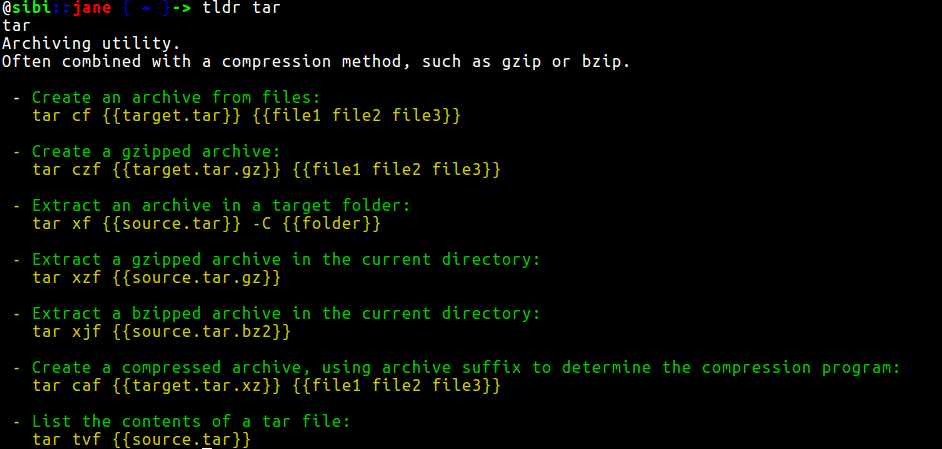
\includegraphics[width=\linewidth]{tldr.png}
  \label{fig:tldr-client}
\end{figure}

Compared to the previous version, the new verion works in Windows and
doesn't do eager cloning. Also default completion support has been
added from optparse-applicative. The new-format branch contains
changes for the new syntax of TLDR pages and will be merged with
master whenever the upstream changes are finalized and merged.

\FurtherReading
  \url{https://github.com/psibi/tldr-hs}
\end{hcarentry}

\end{document}
